\section{The Sosiogram}
During the project the facilitators went around to the groups, analyzing the communication flow within the team during a discussion. They made a sosiogram of it by drawing lines to represent whenever someone talked to individuals or the group as a whole, as we can see in the sosiogram from our group, seen in \autoref{fig:sosiogram}. This sosiogram was made while we had one of our mid-day meetings. None of the group members knew that they were being facilitated. Note that when someone talked to the group in general, it's represented as a line towards the center dot of the "table".

The sosiogram showed that the communication flow had broken down, i.e. some people were hardly involved in the discussion at all, and this was a surprise to us. Hanne, one of the most active participants, was surprised she did not notice that Eirik and Marius were not participating in the discussion, as she had felt that all the members were contributing. Marius was one of the members focused on doing research on the computer during the meeting. He was also surprised over the sociogram because he felt that he could do research and contribute in the group meeting at the same time. On the contrary the sosiogram shows that the members that had their computers up were almost absent from the discussion.

One of the big advantages of a group project is that you get different points of view and constructive criticism of your ideas, so this is something we did not want. Since the sociogram showed that everyone was about as active as the others, with exception of those using their laptop, we decided to add a norm saying that from now on every meeting shall be pc-free, with the exception of the secretary. 

We managed to keep this norm for the rest of the project and we felt that it improved our creativity and productivity. It is hard to measure, but one thing we noticed was that we did not have to repeat the same topics that had been discussed earlier because all group members paid attention and focused on the meeting. 

%The interesting thing about this sosiogram was that all the group members were surprised by how the communication flow had broken down, i.e. some people were far more active in the discussion than others. The group tried to analyse why this had happened and we believe that this was caused by Eirik and Marius having their computers up. The computers first came up to find some information for the discussion, but stayed up longer than necessary and were a distraction.
%Hanne was one of the most active in the group. She was surprised that she didn't notice that  Marius and Erik wasn’t participating in the discussion. She felt that all members were contributing. Marius was one of the members that were focused on doing research on the computer while the group had a meeting. He was also surprised over the sociogram because he felt that he could do research at the same time as contributing in the group meeting. 

%From the sociogram the group reached the conclusion that the two people sitting on their laptop during the meeting, even though they were doing work relevant for the project, was much less active in the discussion. Since one of the big advantages of a group project is that you get different points of view and can have a discussion about the subject the group decided that this was something we didn't want. We wanted to see the effect of interdisciplinary backgrounds. Since the sociogram showed that everyone was about as active as the others, with exception of those using their laptop , we decided to add a norm saying that from now on every meeting shall be pc-free, unless someone was specifically asked to either take notes as a secretary, or check something that we would need in the discussion.

%We managed to keep this norm for the rest of the project and we felt that it improved our creativity and productivity. It is hard to measure it, but the thing we noticed was that we didn't have to repeat the same topics that had been discussed earlier because all group members paid attention and focused on the meeting. 
\begin{figure}
	\begin{center}
		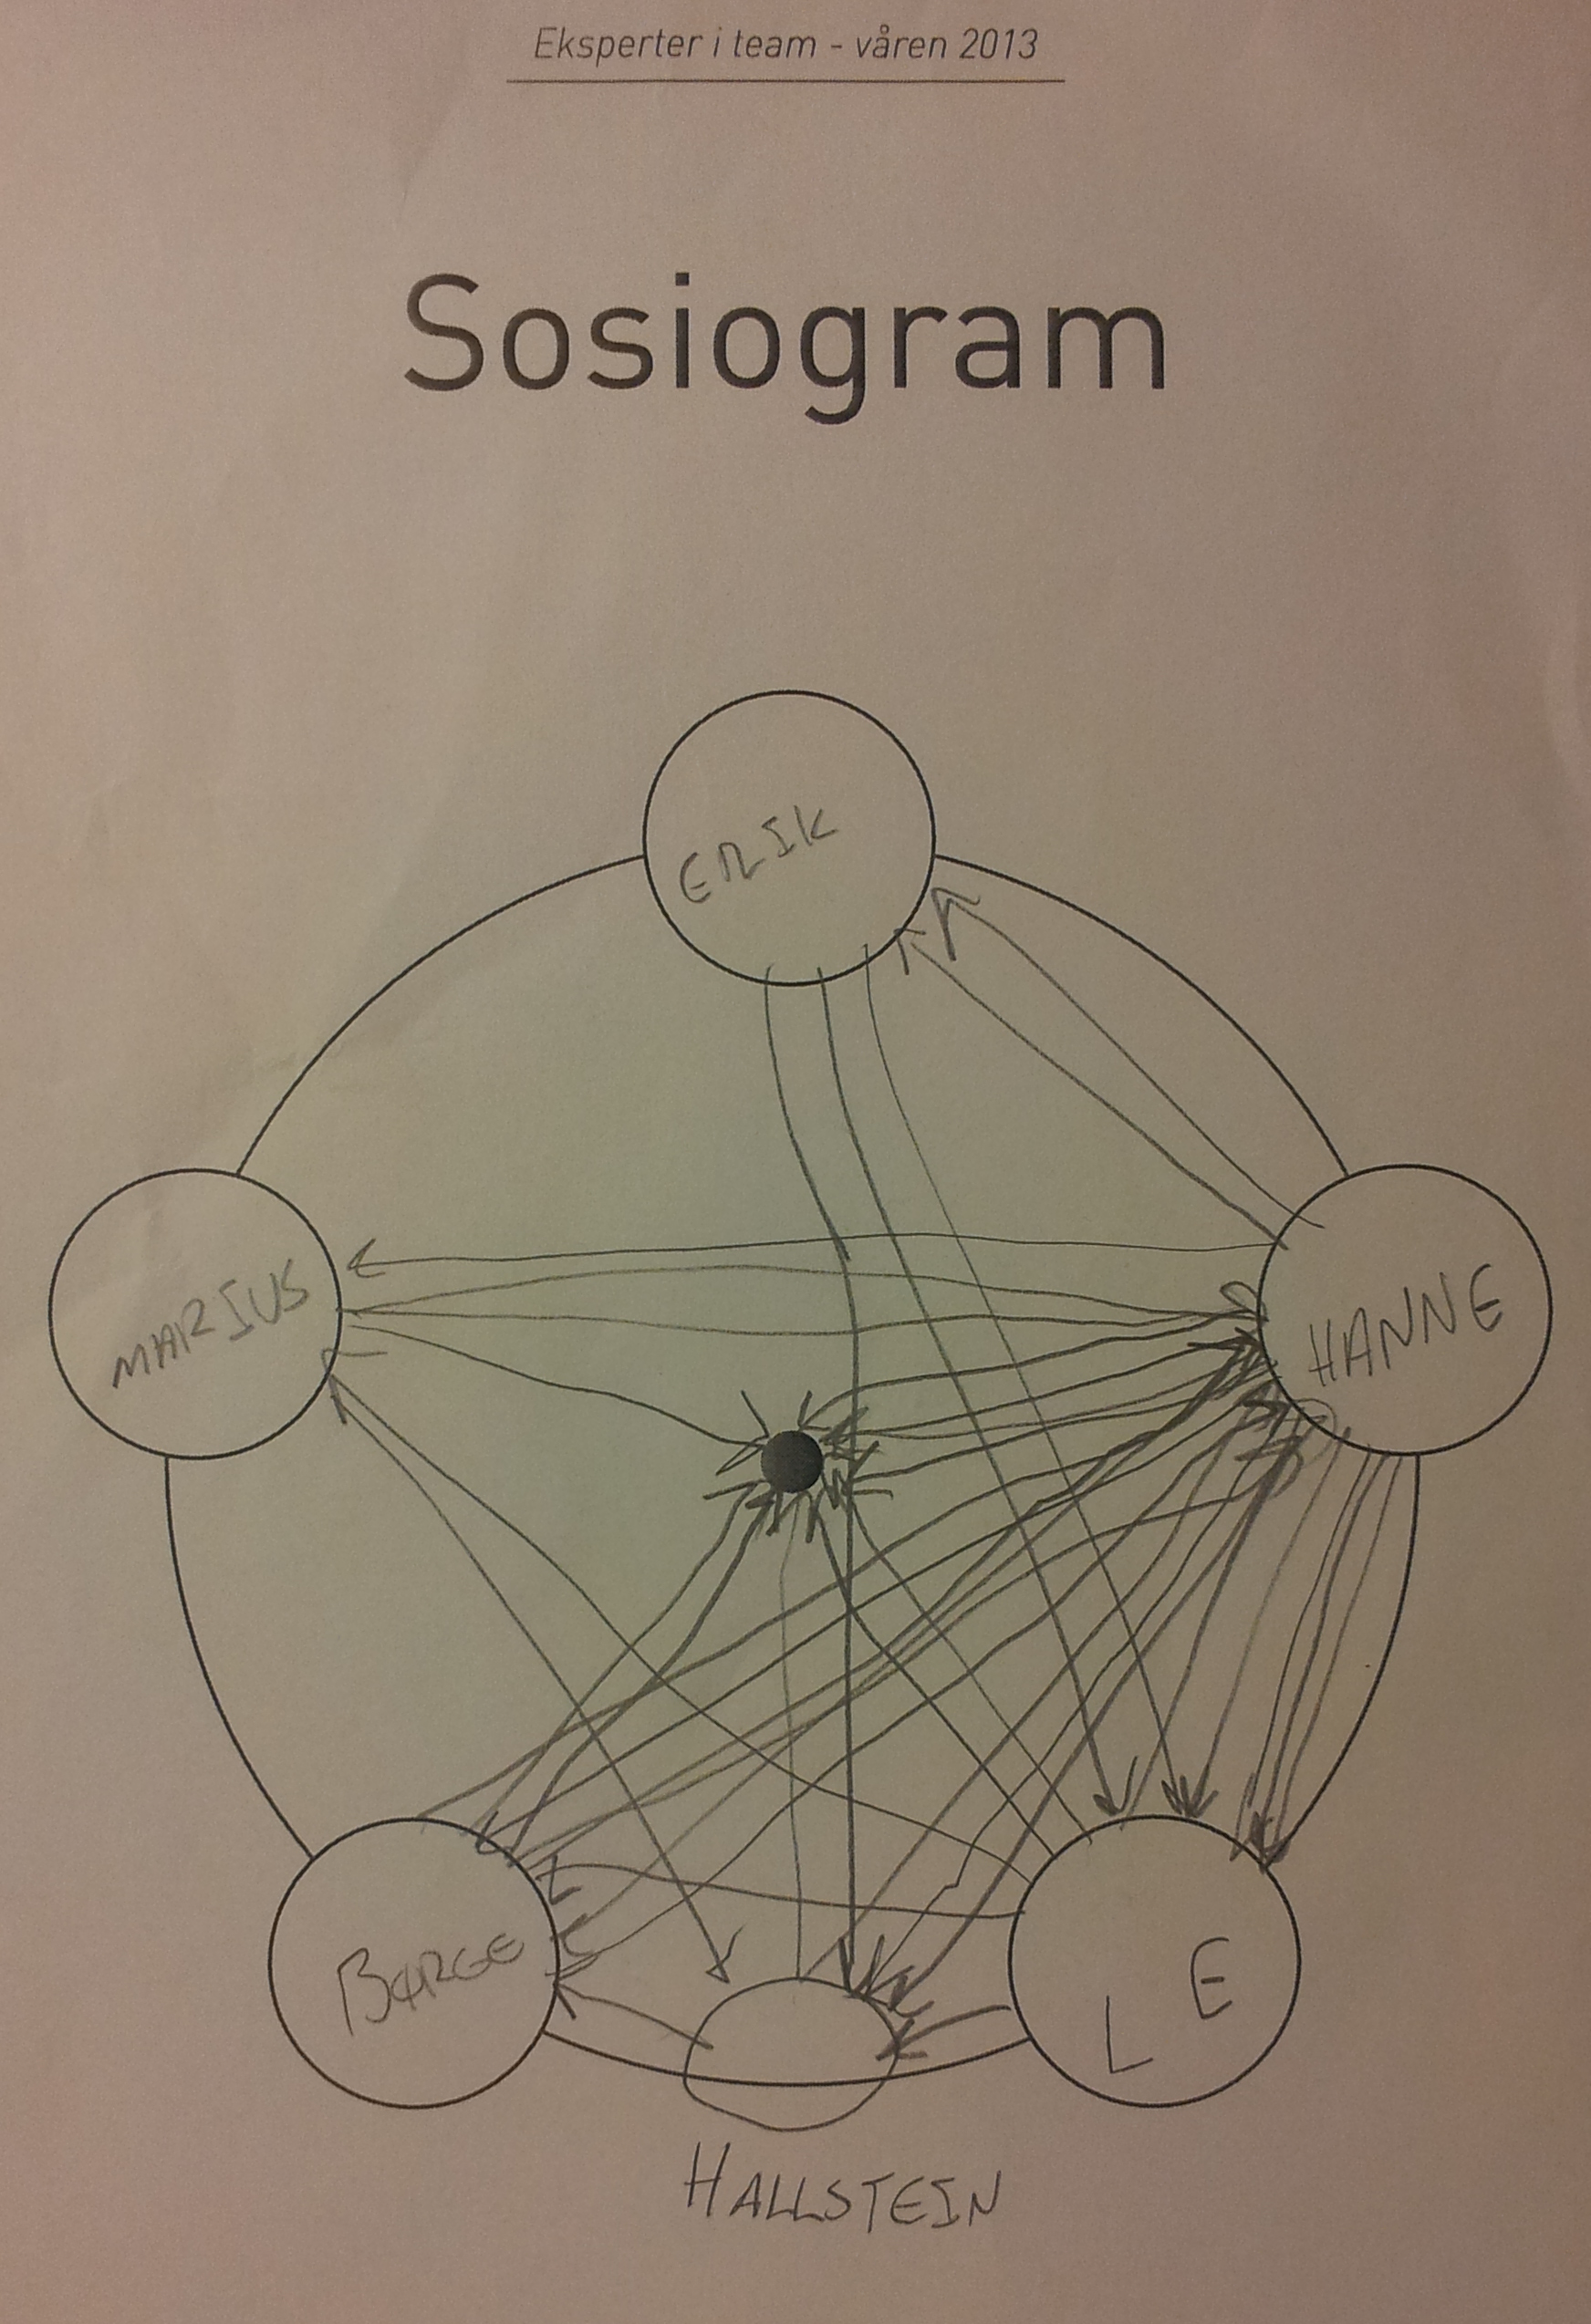
\includegraphics[trim = 10mm 10mm 10mm 250mm, clip, width=0.7\textwidth]{Figures/sosiogram.png}
	\end{center}
	\caption[The Sosiogram]{The Sosiogram we got from the facilitators after they observed a discussion in the group}
	\label{fig:sosiogram}
\end{figure}